\documentclass[12pt,compress,aspectratio=169]{beamer}
\usetheme{metropolis}
\setbeamersize{text margin left=.5cm,text margin right=.5cm}
\usepackage[lf]{carlito}
\usepackage{siunitx}
\usepackage{tikz}
\usepackage{mathpazo}
\usepackage{bm}
\usepackage{mathtools}
\usepackage[ISO]{diffcoeff}
\diffdef{}{ op-symbol=\mathsf{d} }
\usepackage{xcolor,colortbl}

\setmonofont{Ubuntu Mono}
\setlength{\parskip}{0pt}
\renewcommand{\baselinestretch}{1}

\sisetup{
  inter-unit-product=\cdot,
  per-mode=symbol
}

\tikzset{
  >=latex
}

%\newcommand{\iii}{\hat{\bm\imath}}
%\newcommand{\jjj}{\hat{\bm\jmath}}
%\newcommand{\kkk}{\hat{\bm k}}


\setlength{\parskip}{0pt}
\renewcommand{\baselinestretch}{1}

\sisetup{
  inter-unit-product=\cdot,
  per-mode=symbol
}
\tikzset{>=latex}

\title{Topic 15: Light Waves and Optics}
\subtitle{AP (2) and IBHL Physics}
\author[TML]{Dr.\ Timothy Leung}
\institute{Olympiads School}
\date{Updated: Summer 2022}

\newcommand{\pic}[2]{
  \includegraphics[width=#1\textwidth]{#2}
}
\newcommand{\eq}[2]{
  \vspace{#1}{\Large
    \begin{displaymath}
      #2
    \end{displaymath}
  }
}
%\newcommand{\iii}{\ensuremath\hat{\bm{\imath}}}
%\newcommand{\jjj}{\ensuremath\hat{\bm{\jmath}}}
%\newcommand{\kkk}{\ensuremath\hat{\bm{k}}}
\newcommand{\iii}{\ensuremath\hat\imath}
\newcommand{\jjj}{\ensuremath\hat\jmath}
\newcommand{\kkk}{\ensuremath\hat k}



\begin{document}

\begin{frame}
  \maketitle
\end{frame}



\section{Reflection and Refraction}

\begin{frame}{Reflection and Refraction}
  We begin with a model of a beam of light traveling toward an interface
  between two ``indexed material'':
  \begin{center}
    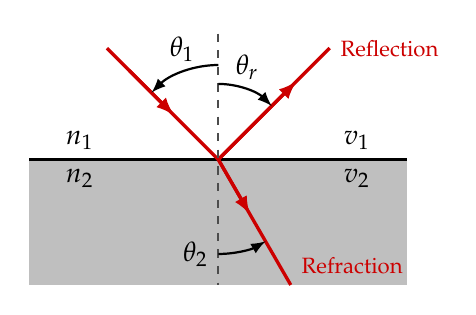
\begin{tikzpicture}[scale=.8]
      \fill[gray!50](-3,-2) rectangle (3,0);
      \draw[very thick](-3,0)--(3,0);
      \begin{scope}[rotate=45,red!80!black,very thick]
        \draw[->](0,2.5)--(0,1);
        \draw (0,2)--(0,0);
        \draw(0,0)--(2.5,0) node[right]{\footnotesize Reflection};
        \draw[->](0,0)--(1.75,0);
      \end{scope}
      \draw[rotate=30,red!80!black,very thick](0,0)--(0,-2.3)
      node[above right]{\footnotesize Refraction};
      \draw[rotate=30,->,red!80!black,very thick](0,0)--(0,-1);
      \draw[dashed,black!70,thick](0,2)--(0,-2);
      \begin{scope}[->,thick]
        \draw (0,1.5) arc(90:135:1.5)  node[midway,above]{$\theta_1$};
        \draw (0,1.2) arc(90:45:1.2)   node[midway,above]{$\theta_r$};
        \draw (0,-1.5)arc(270:300:1.5) node[pos=0,left]  {$\theta_2$};
      \end{scope}
      \node[above] at (-2.2,0) {$n_1$};
      \node[below] at (-2.2,0) {$n_2$};
      \node[above] at (2.2,0)  {$v_1$};
      \node[below] at (2.2,0)  {$v_2$};
    \end{tikzpicture}
  \end{center}
  The \textbf{index of refraction} (or \textbf{refractive index},
  \textbf{index}) of the two media is defined as the ratio of speeds of
  light in a vacuum $c_0$ and in the medium $c$:

  \eq{-.2in}{
    n=\frac{c_0}c\geq 1
  }
\end{frame}

\begin{frame}{Reflection of Light}
  In the \textbf{law of reflection}, the incident ray, the reflected ray, and
  the normal to the surface of the mirror all lie in the same plane, and the
  angle of reflection $\theta_r$ is equal to the angle of incidence $\theta_1$:

  \eq{-.25in}{
    \boxed{\theta_r=\theta_1}
  }
  
  \begin{center}
    \vspace{-.2in}
    \pic{.6}{graphics/Types-of-reflection}
  \end{center}
\end{frame}



\begin{frame}{Specular Reflection Example}
  \begin{center}
    \pic{.55}{graphics/Lake-reflection}
  \end{center}
  This photo of Lake Matheson shows specular reflection in the water of the
  lake with reflected images of Aoraki/Mt Cook (left) and Mt Tasman (right).
  The very still lake water provides a perfectly smooth surface for this to
  occur.
\end{frame}


\begin{frame}{Intensity of Light Reflecting from}
  When the incident and reflected angles normal, i.e.
  $\theta_1=\theta_r=\ang{0}$, the reflected intensity of light $I$ is related
  to the incident intensity $I_0$ by the indices of the two material ($n_1$ and
  $n_2$):

  \eq{-.25in}{
    I=\left[\frac{n_1-n_2}{n_1+n_2}\right]^2 I_0
  }
  
  The intensity of a wave is the power $P$ over the area $A$ that the wave
  passes through:

  \eq{-.2in}{
    I=\frac{P}A
  }

  The reflected intensity is lower than the incident, indicating that some of
  the energy from the incident wave is transmitted into the second medium.
\end{frame}



\begin{frame}{Refraction of Light Through a Medium}
  \textbf{Refraction} occurs when light is transmitted from one medium to
  another at an oblique angle. The wave changes direction due to the difference
  in the speed of light in the two media.
  \begin{center}
    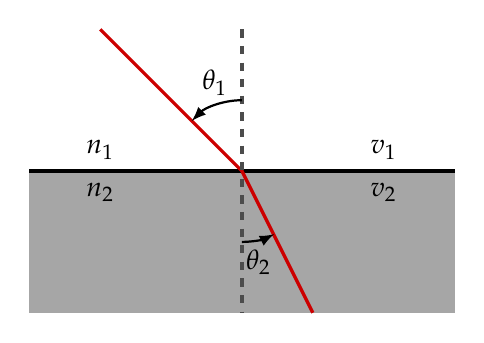
\begin{tikzpicture}[scale=.9]
      \fill[gray!70](-3,-2) rectangle (3,0);
      \draw[very thick](-3,0)--(3,0);
      \draw[red!80!black,very thick](-2,2)--(0,0)--(1,-2);
      \draw[dashed,black!70,very thick](0,2)--(0,-2);
      \draw[->,thick](0,1) arc(90:135:1) node[midway,above]{$\theta_1$};
      \draw[->,thick](0,-1)arc(270:297:1) node[midway,below]{$\theta_2$};
      \node at (-2,.3) {$n_1$};
      \node at (-2,-.3){$n_2$};
      \node at (2,.3) {$v_1$};
      \node at (2,-.3){$v_2$};
    \end{tikzpicture}
  \end{center}
\end{frame}



\begin{frame}{Law of Refraction}
  \textbf{Snell's law} (or \textbf{law of refraction}) relates the refractive
  indices $n$ of the two media to the directions of propagation in terms of the
  angles $\theta$ to the normal

  \eq{-.2in}{
    \boxed{n_1\sin\theta_1=n_2\sin\theta_2}
  }

  This equation holds for the refraction of any kind of wave incident on a
  boundary surface separating two media (e.g.\ surface ocean wave at two
  depths)
\end{frame}



%\begin{frame}{Refraction and Huygens Principle}
%  \begin{columns}
%    \column{.5\textwidth}
%    \pic{1}{graphics/huygen}
%    
%    \column{.5\textwidth}
%    We can explain the refraction phenomenon using Huygens' Principle
%  \end{columns}
%\end{frame}



\begin{frame}{Index of Refraction}
  When light enters a new medium, the \emph{frequency} remains the same: the
  atoms in the new medium would absorb and then radiate the light at the same
  frequency. However, the \emph{speed} of the radiated wave is different,
  therefore a different \emph{wavelength} is observed:
    
  \eq{-.2in}{
    \boxed{\frac{n_1}{n_2}=\frac{\lambda_2}{\lambda_1}}
  }

  You can work this out using the relationship between wave speed, frequenc
  and wavelength: $v=f\lambda$
\end{frame}



\begin{frame}{Index of Refraction of Common Materials}
  \begin{center}
    \begin{tabular}{c|c||c|c}
      \rowcolor{pink}
      \textbf{Material} & $\bm{n}$ & \textbf{Material} & $\bm{n}$\\ \hline
      Vacuum           & 1        & Ethanol     & 1.362 \\
      Air              & 1.000277 & Glycerine   & 1.473 \\
      Water at \SI{20}{\celsius} & 1.33 & Ice         & 1.31 \\
      Carbon disulfide & 1.63     & Polystyrene & 1.59 \\
      Methylene iodide & 1.74     & Crown glass & 1.50-1.62\\
      Diamond          & 2.417    & Flint glass & 1.57-1.75\\
    \end{tabular}
  \end{center}
  The values given are \emph{approximate} and do not account for the small
  variation of index with light wavelength. That's called \textbf{dispersion}.
\end{frame}



\begin{frame}{Total Internal Reflection}
  \textbf{Total internal reflection} (``TIR'') can occur when light enters from
  a medium with high index to another with low index (i.e.\ $n_1>n_2$).
  \begin{center}
    \pic{.55}{graphics/660px-RefractionReflextion}
  \end{center}
  The \textbf{critical angle} can be found for when the refracted angle is
  \ang{90}:

  \eq{-.2in}{
    \boxed{\theta_c=\sin^{-1}\left(\frac{n_2}{n_1}\right)}
  }
  For water-air interface, $\theta_c$=\ang{48.6}
\end{frame}



\begin{frame}{Color of Light and Wavelength}
  Human eyes perceive different frequencies of light as different colors. The
  visible spectrum of light range from about \SI{380}{\nano\metre} (violet) to
  about \SI{700}{\nano\metre} (red).
  \begin{center}
    \pic{.6}{graphics/electromagneticspectrum-141b490bac872789434}
  \end{center}
  A good question to ask: where is \emph{purple}?
\end{frame}



\begin{frame}{Dispersion of Light}
  The index of refraction of a material varies slightly with wavelength
  $\lambda$. This is called \textbf{dispersion}. The dispersion of light
  through a prism is why we can see the rainbow colors from a beam of white
  light:
  \begin{center}
    \pic{.3}{graphics/Prism_rainbow_schema}
  \end{center}
  The index of refraction for shorter wavelengths is always higher than for
  longer wavelengths.
\end{frame}



\begin{frame}{Wavelength Dependency of Index of Refraction}
  We can see that for different kinds of glass, the index of refraction can vary
  significantly through the visible spectrum.
  \begin{center}
    \pic{.4}{graphics/Dispersion-curve}
  \end{center}
\end{frame}



\section{Lenses and Mirrors}

\begin{frame}{Spherical Mirror}
  \begin{columns}
    \column{.6\textwidth}
    We can imagine a \textbf{spherical mirror} to be a sphere with smooth
    light-reflecting surfaces inside and out.
    \begin{itemize}
    \item A \textbf{concave mirror} is the surface \emph{inside} the spherical
      mirror
    \item A \textbf{convex mirror} is the surface \emph{outside} the spherical
      mirror
    \end{itemize}
    \column{.4\textwidth}
    \pic{1}{graphics/spherical-mirror}
  \end{columns}
\end{frame}



\begin{frame}{Spherical Mirror}
  The cross-section diagram of the mirror:
  \begin{center}
    \begin{tikzpicture}[scale=.95]
      \draw[thick,blue](-3,0)--(5.5,0)
      node[pos=.85,above]{\footnotesize principal axis};
      \draw[thick](3,0) arc(0: 30:3);
      \draw[thick](3,0) arc(0:-30:3) node[below]{\footnotesize mirror};
      \fill(0,0) circle(.05) node[below]{\footnotesize $C$};
      \fill(3,0) circle(.05) node[below right]{\footnotesize $V$};
      \draw[rotate=20,->](0,0)--(3,0) node[midway,above]{\footnotesize $R$};
    \end{tikzpicture}
  \end{center}
  \begin{itemize}
  \item\textbf{Center of curvature} $C$: center of the imaginary sphere
    with the same radius as the mirror
  \item\textbf{Radius of curvature} $R$ is any straight line from the
    center of curvature to the curved surface
  \item\textbf{Vertex} $V$ is the geometric center of the mirror surface
  \item\textbf{Principal axis} ``PA'': a straight that passes through $V$ and
    $C$
  \end{itemize}
\end{frame}


\begin{frame}{Spherical vs.\ Parabolic Mirror}
  \begin{itemize}
  \item Rays that are closed to the PA are called \textbf{paraxial rays}; they
    converge at a single point called the \textbf{focal point} $F$
  \item Rays that are far away from the PA are called \textbf{nonparaxial rays};
    they converge to different points
  \end{itemize}
  \begin{center}
    \pic{.6}{graphics/spherical-vs-parabolic}
  \end{center}
  In order for all beams of light to converge to the focal point, a
  \textbf{parabolic mirror} must be used instead of a spherical mirror.
\end{frame}



\begin{frame}{Focal Point and Focal Length}
  The focal point $F$ is exactly half way between the center of curvature and
  the mirror, and the distance to the mirror is called the \textbf{focal length}
  $f$:

  \eq{-.2in}{
    \boxed{f=\frac12 r}
  }
  \begin{center}
    \begin{tikzpicture}
      \draw(-3,0)--(3.5,0) node[right]{\footnotesize PA};
      \draw(3,0) arc(0: 30:3);
      \draw(3,0) arc(0:-30:3) node[below]{\footnotesize mirror};
      \fill(0,0) circle(.05) node[below]{\footnotesize $C$};
      \fill(3,0) circle(.05) node[below right]{\footnotesize $V$};
      \fill[red](1.5,0) circle(.05) node[above]{\footnotesize $F$};
      \draw[red,<->,thick](1.5,0)--(3,0) node[midway,below]{\footnotesize $f$};
      \draw[rotate=20,->](0,0)--(3,0) node[midway,above]{\footnotesize $R$};
    \end{tikzpicture}
  \end{center}
  
\end{frame}


\begin{frame}{Mirror Equation}
  In terms of the focal length, the \textbf{mirror equation} is expressed as

  \eq{-.2in}{
    \boxed{\frac1s+\frac1{s'}=\frac1f}
  }
  \begin{center}
    \begin{tabular}{l|c|c}
      \rowcolor{pink}
      \textbf{Quantity} & \textbf{Symbol} & \textbf{SI Unit} \\ \hline
      Distance to object & $s$  & \si{\metre} \\
      Distance to image  & $s'$ & \si{\metre} \\
      Focal length       & $f$  & \si{\metre} 
    \end{tabular}
  \end{center}
  This equation is derived mathematically using basic geometry and the
  small-angle approximation.
\end{frame}



\begin{frame}{Sign Convention for the Mirror Equation}
  When working with the mirror equation, we use the following sign convention:
  
  \eq{-.2in}{
    \boxed{\frac1s+\frac1{s'}=\frac1f}
  }
  \begin{center}
    \begin{tabular}{ccl}
      \hline
      $s$ & $+$ & object is in front of the mirror (real object) \\
      & $-$ & object is behind the mirror (virtual object)\\\hline
      $s'$ & $+$ & image is in front of the mirror (real image)\\
      & $-$ & image is in behind the mirror (virtual image)\\\hline
      $R$, $f$ & $+$ & center of curvature is in front of the mirror
      (concave mirror)\\
      & $-$ & center of curvature is behind the mirror (convex mirror)\\
      \hline
    \end{tabular}
  \end{center}
\end{frame}



\begin{frame}{Lateral Magnification}
  Using the sign convention as the mirror equation, the
  \textbf{lateral magnification} of the object is given by:

  \eq{-.2in}{
    \boxed{m=\frac{h'}h=-\frac{s'}s}
  }
  \begin{center}
    \begin{tabular}{l|c|l}
      \rowcolor{pink}
      \textbf{Quantity} & \textbf{Symbol} & \textbf{SI Unit} \\ \hline
      Magnification factor & $m$ & (no units)\\
      Object \& image height & $h$, $h'$  & \si{\metre} (metres)\\
      Distance to object \& image & $s$, $s'$  & \si{\metre} (metres)
    \end{tabular}
  \end{center}
  \begin{itemize}
  \item $m>0$:image is upright; $m<0$: image is inverted
  \item $|m|>1$: image is enlarged; $|m|<1$: image is reduced
  \item If both $s$ and $s'$ are positive (on the same side), then the image
    is inverted
  \end{itemize}
\end{frame}



\begin{frame}{Geometry of Convex Lenses}
  Here are some defining geometric properties for the \textbf{thin lens}.
  \begin{center}
    \pic{.5}{graphics/thin-lens}
  \end{center}
  The surface that light first passes through has the radius $R_1$ while the
  second surface has $R_2$.
\end{frame}



\begin{frame}{Focal Length of the Thin Lens}
  The focal length $f$ of a thin lens is defined using the
  \textbf{lens-makers' equation}:

  \eq{-.2in}{
    \boxed{\frac1f=(n-1)\left(\frac1{R_1}-\frac1{R_2}\right)}
  }
  \begin{center}
    \begin{tabular}{l|c|c}
      \rowcolor{pink}
      \textbf{Quantity} & \textbf{Symbol} & \textbf{SI Unit} \\ \hline
      Focal length                    & $f$ & (no units)\\
      Index of refraction of the lens & $n$ & \si{\metre} \\
      Radii of curvature              & $R_1$, $R_2$ & \si{\metre}
    \end{tabular}
  \end{center}  
\end{frame}



\begin{frame}{Thin Lens Equation}
  The \textbf{thin-lens equation} is exactly the same as the mirror equation:

  \eq{-.2in}{
    \boxed{\frac1s+\frac1{s'}=\frac1f}
  }
  \begin{center}
    \begin{tabular}{l|c|c}
      \rowcolor{pink}
      \textbf{Quantity} & \textbf{Symbol} & \textbf{SI Unit} \\ \hline
      Distance to object & $s$  & \si{\metre} \\
      Distance to image  & $s'$ & \si{\metre} \\
      Focal length       & $f$  & \si{\metre}
    \end{tabular}
  \end{center}
\end{frame}



\begin{frame}{Sign Convention for the Thin Lens Equation}
  When working with the thin-lens equation, we use the following sign
  convention:
  
  \eq{-.2in}{
    \boxed{\frac1s+\frac1{s'}=\frac1f}
  }
  \begin{center}
    \begin{tabular}{ccl}
      \hline
      $s$ & $+$ & real object: for objects in front of the lens (incident
      side) \\
      & $-$ & virtual object: for objects behind the lens (transmission side)
      \\\hline
      $s'$ & $+$ & real image: behind the lens (transmission side)\\
      & $-$ & virtual image: in front of the lens (virtual image)\\\hline
      $R$, $f$ & $+$ & center of curvature is on the transmission side\\
      & $-$ & center of curvature on the incident side\\
      \hline
    \end{tabular}
  \end{center}
\end{frame}



\begin{frame}{Lateral Magnification}
  Likewise, the  \textbf{lateral magnification} of the image is given by the
  same equation as the mirror, but this time using the sign convention for
  the thin lens:

  \eq{-.2in}{
    \boxed{m=\frac{h'}h=-\frac{s'}s}
  }
  \begin{center}
    \begin{tabular}{l|c|c}
      \rowcolor{pink}
      \textbf{Quantity} & \textbf{Symbol} & \textbf{SI Unit} \\ \hline
      Magnification factor & $m$ & (no units)\\
      Object height & $h$  & \si{\metre} \\
      Image height  & $h'$ & \si{\metre} \\
      Distance to object & $s$  & \si{\metre} \\
      Distance to image  & $s'$ & \si{\metre}
    \end{tabular}
  \end{center}
\end{frame}




\section{Interference of Light}

\begin{frame}{Thomas Young's Double-Slit Experiment}
  \begin{columns}
    \column{.45\textwidth}
    \pic{1}{graphics/double-slit1}
    
    \column{.52\textwidth}
    \begin{itemize}
    \item\textbf{Monochromatic light} light with a single color (frequency);
      the light source can be a laser, LED , or gas lamp (most likely what Young
      used)
    \item\textbf{Slit:} an opening; also called an \textbf{aperture}
    \item The \textbf{screen} far away from the slits is also called the
      \textbf{projection}
    \end{itemize}
  \end{columns}

  \vspace{.15in}Double-slit experiment showed that light causes interference,
  just like any other wave
\end{frame}

\begin{frame}{Thomas Young's Double-Slit Experiment}
  \begin{columns}
    \column{.28\textwidth}
    \pic{1.15}{graphics/path1}
    
    \column{.72\textwidth}
    \begin{itemize}
    \item At \textbf{A}, the path from slits $S_1$ and $S_2$ are the same,
      therefore we have \textbf{constructive interference} and the projection
      is bright
    \item At \textbf{B}, the path from $S_1$ and $S_2$ are diffed by half a
      wavelength, and therefore there is \textbf{destructive interference} and
      the projection is dark
    \item At \textbf{C}, the path from $S_1$ and $S_2$ are diffed by one
      wavelength, and therefore there is \textbf{constructive interference}
      again, and again, the projection is bright
    \end{itemize}
  \end{columns}
\end{frame}



\begin{frame}{Interference Pattern: Bright and Dark Fringes}
  \begin{center}
    \pic{.4}{graphics/fringes1}
  \end{center}
  The ``bright fringes'' are from constructive interference; the ``dark
  fringes'' are from destructive interference.
\end{frame}



\begin{frame}{Geometry of the Two-Slit Interference}
  Two coherent (in phase) sources pass through two narrow slits (that can be
  treated as point sources). The light from the slits emerge at the screen $P$
  at a distance $L$ away.
  \begin{center}
    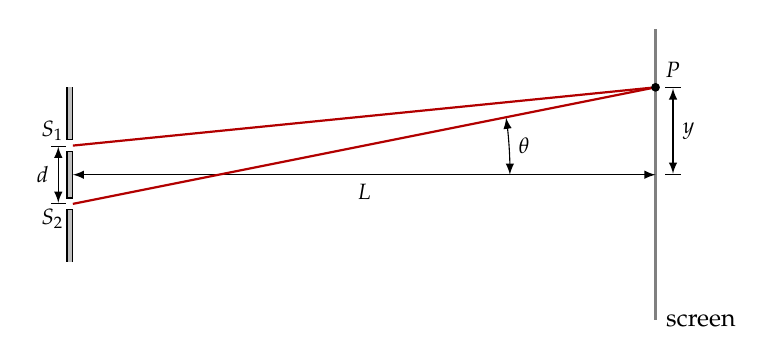
\begin{tikzpicture}[scale=.37]
      % Draw the slits
      \draw[fill=gray!50](0,3)--(0,1.2)--(-0.2,1.2)--(-0.2,3);
      \draw[fill=gray!50](0,0.8)--(0,-0.8)--(-0.2,-0.8)--(-0.2,0.8)--cycle;
      \draw[fill=gray!50](0,-3)--(0,-1.2)--(-0.2,-1.2)--(-0.2,-3);
      \draw[|<->|](-0.5,-1)--(-0.5,1) node[midway,left]{\footnotesize $d$};
      \node at (-.7,1.5) {\footnotesize $S_1$};
      \node at (-.7,-1.5) {\footnotesize $S_2$};
      %\draw[thin,gray!30] (0,0) circle(2.8);
      
      % Draw the screen
      \draw[line width=1pt,gray](20,5)--(20,-5)node[right,black]{\small screen};

      % Draw dimension of the problem
      \draw[<->](0,0)--(20,0) node[midway,below]{\footnotesize $L$};
      \draw[|<->|](20.6,0)--(20.6,3) node[midway,right]{\footnotesize $y$};
      % Draw rays to P
      \draw[red!70!black,thick](0,1)--(20,3);
      \draw[red!70!black,thick](0,-1)--(20,3);
      \draw[<->](15,0) arc(0:7.5:15) node[midway,right]{\footnotesize $\theta$};
      \fill[black](20,3) circle(.15) node[above right]{\footnotesize $P$};
    \end{tikzpicture}
  \end{center}
  \vspace{-.1in}The two beams travel a slightly different distance:
  \begin{itemize}
  \item\textbf{Constructive interference:} path difference is an integer
    multiple  of $\lambda$
  \item\textbf{Destructive interference:} path difference is a half-integer
    multiple  of $\lambda$
  \end{itemize}
\end{frame}



\begin{frame}{Geometry of the Two-Slit Interference}
  Using basic geometry, we can see that the path difference from the
  two slit to the projection is $d\sin\theta$.
  \begin{columns}
    \column{.35\textwidth}
    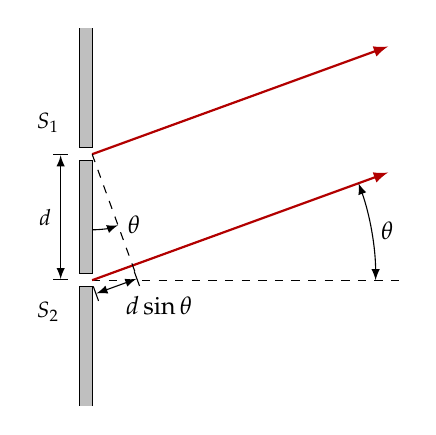
\begin{tikzpicture}[scale=.8]
      % Draw the slits
      \draw[fill=gray!50](0,3)--(0,1.1)--(-.2,1.1)--(-.2,3);
      \draw[fill=gray!50](0,.9)--(0,-.9)--(-.2,-.9)--(-.2,.9)--cycle;
      \draw[fill=gray!50](0,-3)--(0,-1.1)--(-.2,-1.1)--(-.2,-3);
      \draw[|<->|](-.5,-1)--(-.5,1) node[midway,left]{\footnotesize $d$};
      \node at (-.7,1.5) {\footnotesize $S_1$};
      \node at (-.7,-1.5) {\footnotesize $S_2$};
      \draw[dashed](0,-1)--(5,-1);
      \begin{scope}[rotate around={20:(0,-1)}]
        \draw[->,thick,red!70!black](0,-1)--(5,-1);
      \end{scope}
      \begin{scope}[rotate around={20:(0,1)}]
        \draw[->,thick,red!70!black](0,1)--(5,1);
        \draw[dashed](0,1)--(0,-1);
        \draw[|<->|](0,-1.1)--(-.71,-1.1)
        node[midway,below right]{\small$d\sin\theta$};
        \draw[<-](0,-.2) arc(270:250:1.2) node[pos=0,right]{\small$\theta$};
      \end{scope}
      \draw[<->](4.5,-1) arc(0:20:4.5) node[midway,right]{\small$\theta$};
    \end{tikzpicture}

    \column{.65\textwidth}
    \textbf{Constructive maxima} occur when:

    \eq{-.3in}{
      \boxed{n\lambda = d\sin\theta_n}
    }

    \textbf{Destructive minima} occur when:
  
    \eq{-.2in}{
      \boxed{\left(n+\frac12\right)\lambda = d\sin\theta_n}
    }
    \begin{itemize}
    \item\vspace{-.1in}$n=0,1,2,3\ldots n_\text{max}$ is called the
      \textbf{order number}
    \item $n_\text{max}$ can be found by setting $\sin\theta=1$
    \item The number of maxima is $2n_\text{max}+1$
    \end{itemize}
  \end{columns}
\end{frame}


\begin{frame}{Approximation of The Wavelength of Light}
  For small angles, we can apply the \textbf{small-angle approximation} where

  \eq{-.3in}{
    \sin\theta\approx\tan\theta\approx\theta
  }

  \vspace{-.15in}to find that the $n$-th bright fringe is located at $y_n$,
  which allows us to calculate the distance between fringes $\Delta y$:
  
  \eq{-.2in}{
    \boxed{y_n=n\frac{\lambda L}d}
    \quad\rightarrow\quad
    \boxed{\Delta y=\frac{\lambda L}d}
  }

  This equation is used to estimate the wavelength of light based on
  the distances between bright fringes (or dark fringes).
\end{frame}



\begin{frame}{Important Notes}
  \begin{itemize}
  \item We usually apply the double-slit problem to light, but the problem can
    be applied to any wave (e.g.\ EM waves, sound waves, ocean waves) as well
  \item The sources don't actually need to be slits; any point source will do
  \item The projection/screen doesn't need to be a real screen either; it just
    has to be a line where wave intensity can be measured
  \end{itemize}

  \vspace{.25in}Remember:
  \begin{itemize}
  \item integer multiple = constructive maxima
  \item half-integer multiple = destructive minima
  \end{itemize}
\end{frame}



\begin{frame}{Interference of Multiple Equally Spaced Point sources}
  When there are multiple equally-spaced point sources (e.g.\ diffraction
  grating) we can just use the equation for two-slits:

  \eq{-.25in}{
    n\lambda = d\sin\theta
  }
  \begin{center}
    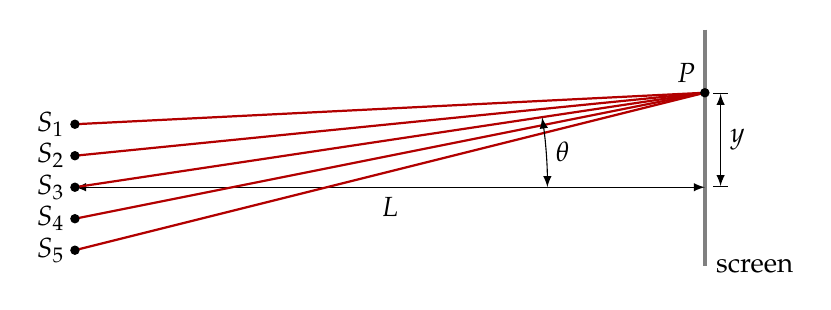
\begin{tikzpicture}[scale=.4]
      % Draw the screen
      \draw[line width=1.5pt,gray](20,5)--(20,-2.5) node[black,right]{screen};

      % Draw dimension of the problem
      \draw[<->](0,0)--(20,0) node[midway,below]{$L$};
      \draw[|<->|](20.5,0)--(20.5,3) node[midway,right]{$y$};
      % Draw rays to P
      \foreach \x in {1,...,5} {
        \draw[red!70!black,thick](0,3-\x)--(20,3)
        node[pos=0,left,black]{$S_{\x}$};
        \fill[black](0,3-\x) circle(.15);
      }
      \draw[<->](15,0) arc(0:8.5:15) node[midway,right]{$\theta$};
      \fill[black](20,3) circle(.15) node[above left]{$P$};
    \end{tikzpicture}
  \end{center}
  The interference pattern gets sharper with increasing number of sources, and
  the bright fringes are narrower.
\end{frame}




\section{Diffraction}

\begin{frame}{Diffraction of Waves}
  When a wave goes through an small opening, it \textbf{diffracts}. This happens
  with sound waves, ocean waves\ldots and light.
  \begin{center}
    \pic{.55}{graphics/alexandria}
  \end{center}
  The photo is from the Port of Alexandria in Egypt. The shape of the entire
  harbor is created because of diffraction of ocean wave.
\end{frame}



\begin{frame}{Diffraction of Waves}
  \begin{center}
    \pic{.6}{graphics/diffraction1}
  \end{center}
  The smaller the opening (compared to the wavelength of the incoming wave)
  the greater the diffraction effects.
\end{frame}


\begin{frame}{Geometry for Single-Slit Diffraction}
  To examine the geometry for the single-slit diffraction problem, we treat
  the wave passing through the slit of width $W$ as an infinite series of point
  sources at the slit.
  
  \vspace{.2in}\begin{columns}
    \column{.4\textwidth}
    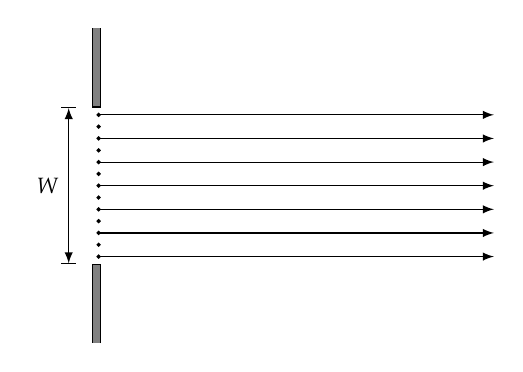
\begin{tikzpicture}
      \draw[fill=gray](0,2)--(0,1)--(-0.1,1)--(-0.1,2);
      \draw[fill=gray](0,-2)--(0,-1)--(-0.1,-1)--(-0.1,-2);
      \draw[|<->|](-.4,-1)--(-.4,1) node[midway,left]{\footnotesize $W$};
      \foreach \y in {1,...,13} {
        \pgfmathsetmacro\yy{1.05-0.15*\y};
        \draw[fill=black](-0.02,\yy) circle(.02);
      }

      \foreach \y in {1,3,...,13} {
        \pgfmathsetmacro\yy{1.05-0.15*\y};
        \draw[->](-0.02,\yy)--(5,\yy);
      }
    \end{tikzpicture}
    
    \column{.6\textwidth}
    \begin{itemize}
    \item Light from the wavelets traveling perpendicular to the aperture do
      not interfere with one another
    \item Therefore, there is a bright fringe at the middle, called the
      \textbf{central diffraction maximum}.
    \end{itemize}
  \end{columns}
\end{frame}




\begin{frame}{Geometry for Single-Slit Diffraction}
  Using the same analysis from the double-slit problem, we find that the path
  difference the wavelets at the top and bottom edges is $W\sin\theta$

  \vspace{.2in}\begin{columns}
    \column{.4\textwidth}
    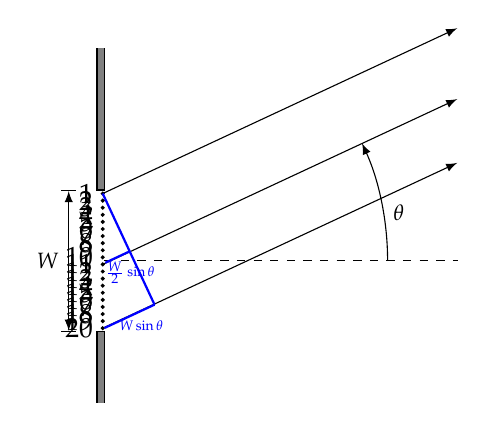
\begin{tikzpicture}[scale=.9]
      \draw[fill=gray](0,3)--(0,1)--(-0.1,1)--(-0.1,3);
      \draw[fill=gray](0,-2)--(0,-1)--(-0.1,-1)--(-0.1,-2);
      \draw[|<->|](-.5,-1)--(-.5,1) node[midway,left]{\footnotesize $W$};
      \foreach \y in {1,...,20} {
        \pgfmathsetmacro\yy{1.05-0.1*\y};
        \draw[fill=black](-0.02,\yy) circle(0.02) node[left]{\Tiny\y};
        }
      \foreach \y in {1,11,20} {
        \pgfmathsetmacro\yy{1.05-0.1*\y};
        \draw[->,rotate around={25:(-0.02,\yy)}](-0.02,\yy)--(5.5,\yy);
      }
      \draw[dashed](0,0)--(5,0);
      \draw[->](4,0) arc(0:24.5:4) node[pos=.4,right]{\footnotesize $\theta$};
      \begin{scope}[rotate around={25:(-0.02,0.95)}]
        \draw[blue,thick](-0.02,0.95)--(-0.02,-0.78);
        \draw[blue,thick](-0.02,-0.78)--(-0.8,-0.78)
        node[pos=.9,right]{\tiny $W\sin\theta$};
        \draw[blue,thick](-0.02,0.05)--(-0.4,0.05)
        node[pos=0,below]{\tiny $\frac{W}2\sin\theta$};
      \end{scope}

    \end{tikzpicture}
    
    \column{0.57\textwidth}
    \begin{itemize}
    \item At some angle $\theta$, the path difference between 1 and 20 will be
      an integer multiple of the wavelength ($m\lambda$)
    \item In this case, the path difference between 1 and 11 is a half-number
      multiple of the wavelength (i.e.\ destructive interference) and they
      cancel each other
    \item Similarly, 2 cancels 12, 3 cancels 13\ldots
    \end{itemize}
    \textbf{RESULT: Complete destructive interference}
  \end{columns}
\end{frame}



\begin{frame}{Geometry for Single-Slit Diffraction}
  \begin{columns}
    \column{.38\textwidth}
    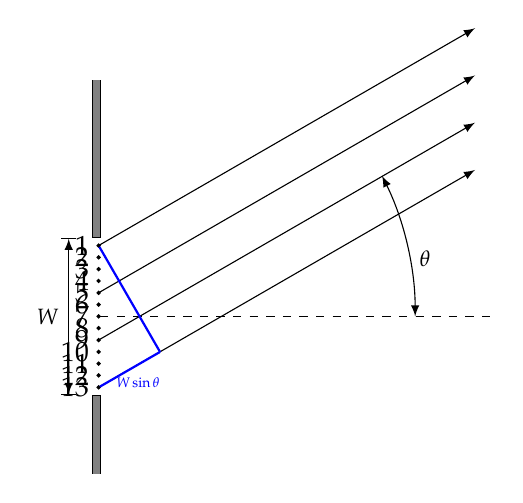
\begin{tikzpicture}
      \draw[fill=gray](0,3)--(0,1)--(-0.1,1)--(-0.1,3);
      \draw[fill=gray](0,-2)--(0,-1)--(-0.1,-1)--(-0.1,-2);
      \draw[|<->|](-.4,-1)--(-.4,1) node[midway,left]{\footnotesize $W$};
      \foreach \y in {1,...,13} {
        \pgfmathsetmacro\yy{1.05-0.15*\y};
        \draw[fill=black](-0.02,\yy) circle(0.02) node[left]{\Tiny\y};
        }
      \foreach \y in {1,5,9,13} {
        \pgfmathsetmacro\yy{1.05-0.15*\y};
        \draw[->,rotate around={30:(-0.02,\yy)}](-0.02,\yy)--(5.5,\yy);
      }
      \draw[dashed](0,0)--(5,0);
      \draw[<->](4,0) arc(0:26.5:4) node[pos=.4,right]{\footnotesize $\theta$};
      
      \begin{scope}[rotate around={30:(-0.02,0.9)}]
        \draw[blue,thick](-0.02,0.88)--(-0.02,-0.66);
        \draw[blue,thick](-0.02,-0.66)--(-.9,-0.66)
        node[pos=.9,right]{\tiny $W\sin\theta$};
      \end{scope}
    \end{tikzpicture}

    \column{.62\textwidth}
    \begin{itemize}
    \item At some other angle $\theta$, the path difference between the top
      and bottom is $W\sin\theta=\dfrac32\lambda$
    \item 1 and 5 differ by $\dfrac{\lambda}2$, so they cancel (as do 2 and 6,
      3 and 7, 4 and 8, 9 and 13)
    \item But some of the beams will not, so we have a ``bright fringe'' at the 
      projection
    \item This bright fringe is not as bright as the central one because
      of the destructive interference
    \end{itemize}
  \end{columns}
\end{frame}



\begin{frame}{Dark and Bright Fringes}
  Destructive mimina exist on the screen at regular, whole-numbered intervals
  ($m=1,2,3\ldots$):

  \eq{-.2in}{
    \boxed{m\lambda=W\sin\theta_m}
  }

  while bright fringes exist on the screen at regular, half-numbered intervals:

  \eq{-.2in}{
    \boxed{\left(m+\frac12\right)\lambda=W\sin\theta_m}
  }

  The equations look very similar to the double-slit equations for, but with
  dark and bright fringes in reverse, so be \emph{very} careful when you use
  them!
\end{frame}



\begin{frame}{Bright and Dark Fringes}
  The location of the bright fringes on the screen is determined by applying
  the small-angle approximation equation:
  
  \eq{-.2in}{
    \boxed{y_m=\left(m+\frac12\right)\frac{\lambda L}W}
  }

  While for the dark fringes, 

  \eq{-.2in}{
    \boxed{y_m=\frac{m\lambda L}W}
  }

  Again, the equations look to be the reverse of the two-slit problem.
\end{frame}



\begin{frame}{Single-Slit Diffraction, A Summary}
  \begin{itemize}
  \item Similar to the double-slit interference, single-slit diffraction
    projects a series of alternating bright fringes (``maxima'') and dark
    fringes (``minima'') in the far field
  \item The bright fringe in the middle (``central diffraction maximum'') is
    twice as wide  and very bright
  \item Subsequent bright fringes on either side (``higher-order maxima'') are
    much dimmer because of the partial destructive interference
  \end{itemize}
  \begin{center}
    \pic{.5}{graphics/Single_Slit_Diffraction}
  \end{center}
\end{frame}



\section{Optical Resolution}

\begin{frame}{Optical Resolution}
  The ability of an optical instrument (e.g.\ the human eye, microscope,
  camera) to distinguish two distinct objects
  \begin{center}
    \pic{.32}{graphics/resolve1}
    \pic{.32}{graphics/resolve2}
    \pic{.32}{graphics/resolve3}
  \end{center}
  When light from any object passes through an ``optical instrument'', it
  \emph{diffracts}, therefore ``blurring'' the object
\end{frame}



\begin{frame}{Optical Resolution}
  \begin{columns}
    \column{.4\textwidth}
    \pic{1}{graphics/resolve4}

    \column{.6\textwidth}
    \textbf{Rayleigh limit}: Two objects are resolved if the angle
      $\theta>\theta_\text{min}$, where $\theta_\text{min}$ is when the first
      minimum (dark fringe) from object 1 overlaps with the central maximum
      (bright fringe in the middle) from object 2.
  \end{columns}
\end{frame}


\begin{frame}{Resolving Power}
  To resolve two objects, the minimum angle between rays from the two objects
  passing through an aperture is given by:
  $D$ of the aperture.
  \vspace{0.2in}
  \begin{columns}
    \column{0.5\textwidth}
    Rectangular aperture:

    \eq{-.2in}{
      \boxed{\theta_\text{min}=\frac{\lambda}W}
    }
    \column{0.5\textwidth}
    Circular aperture:

    \eq{-.2in}{
      \boxed{\theta_\text{min}=\frac{1.22\lambda}D}
    }
  \end{columns}
  where $W$ is the width of the aperture, and $D$ is the diameter of the
  aperture. The angle $\theta_\text{min}$ is measured in \textbf{radians}.
\end{frame}


\section{Thin-Film Interference}

\begin{frame}{Thin-Film Interference}
  \textbf{Thin-film interference} occurs when light reflected/refracted at
  the upper \& lower boundaries of a thin film of an indexed material interfere
  with one another
  \begin{itemize}
  \item ``Indexed material'' means a material that has a refractive index of
    $n>1$
  \item The film is a few wavelengths in thickness
  \item The thickness determines whether the interference is constructive or
    destructive
  \item When white light is incident on the film, some colours are enhanced
    while others are reduced
  \end{itemize}
\end{frame}



\begin{frame}{Thin-Film Interference}
  \begin{center}
    \pic{.4}{soap-bubble}\hspace{.01in}
    \pic{.277}{oil-film}\hspace{.01in}
    \pic{.2265}{camera-lens}
  \end{center}
  Examples:
  \begin{itemize}
  \item Soap bubbles
  \item Oil films on water
  \item Anti-reflection coatings on glasses and camera lenses
  \end{itemize}
\end{frame}



\begin{frame}{Optical Path Difference}
  \begin{columns}
    \column{.3\textwidth}
    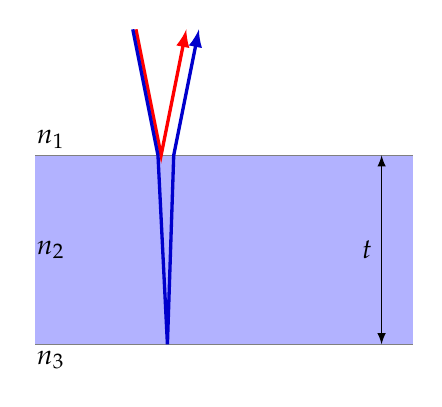
\begin{tikzpicture}[scale=.8]
      \fill[blue!30](0,0) rectangle(6,3);
      \draw[gray](0,0)--(6,0);
      \draw[gray](0,3)--(6,3);
      \draw[<->](5.5,0)--(5.5,3) node[midway,left]{$t$};
      \draw[very thick,red,->](1.6,5)--(2,3)--(2.4,5);
      \draw[very thick,blue!80!black,->]
      (1.55,5)--(1.95,3)--(2.1,0)--(2.2,3)--(2.6,5);
      \node at (.25,1.5 ){$n_2$};
      \node at (.25,3.25){$n_1$};
      \node at (.25,-.25){$n_3$};
    \end{tikzpicture}
    
    \column{.7\textwidth}
    \begin{itemize}
    \item Light hits the upper interface:
      \begin{itemize}
      \item Some light is reflected into the first medium
        (\textcolor{red}{red})
      \item Some light is refracted, then reflected at the lower interface,
        then refracted into the first medium (\textcolor{blue}{blue})
      \end{itemize}
    \item Assuming that the incident and refracted angles are small, then
      optical path difference $\Gamma$ is just:

    \eq{-.25in}{
      \Gamma=2t
    }

    \vspace{-.15in}Same as single- and double-slits interference problems,
    $\Gamma$ determines the condition for constructive and destructive
    interference
    \end{itemize}
  \end{columns}
\end{frame}



\begin{frame}{Optical Path Difference}
  The wavelength in the second medium $\lambda'$ is related to the incident
  wavelength $\lambda$ using the universal wave equation:

  \eq{-.18in}{
    \lambda'=\frac{n_1}{n_2}\lambda
  }
  
  If the first medium is air,  use $n_1=1$ for simplicity
\end{frame}



\begin{frame}{Soap Bubble}
  \begin{center}
    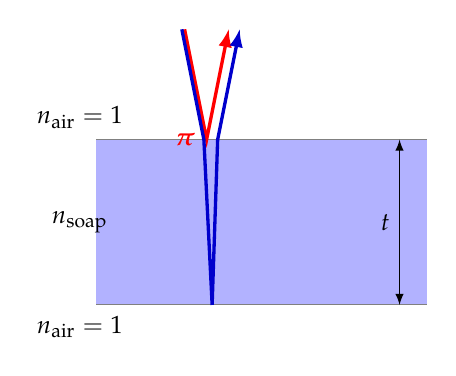
\begin{tikzpicture}[scale=.7]
      \fill[blue!30](0,0) rectangle(6,3);
      \draw[gray](0,0)--(6,0);
      \draw[gray](0,3)--(6,3);
      \draw[<->](5.5,0)--(5.5,3) node[midway,left]{\small  $t$};
      \draw[very thick,red,->]
      (1.6,5)--(2,3) node[left]{\small $\bm{\pi}$}--(2.4,5);
      \draw[very thick,blue!80!black,->]
      (1.55,5)--(1.95,3)--(2.1,0)--(2.2,3)--(2.6,5);
      \node at (-.3,1.5 ){\small $n_\text{soap}$};
      \node at (-.3,3.4){\small $n_\text{air}=1$};
      \node at (-.3,-.4){\small $n_\text{air}=1$};
    \end{tikzpicture}
  \end{center}
  \vspace{-.1in}Light travels through air and strikes a soap film (with
  $n_\text{soap}$). On either side of the soap film is air.
  \begin{itemize}
  \item Upper interface: reflected light has a \ang{180} ($\pi$ radian)
    phase shift, as $n_\text{air}<n_\text{soap}$, i.e.\ light reflects from a
    fast to slow medium
  \item Lower interface: the reflected wave has no phase shift (slow to
    fast medium)
  \end{itemize}
\end{frame}



\begin{frame}{Soap Bubble}{Condition for Interference}
  Because of the phase shift, \emph{constructive maxima} occurs if path
  difference $\Gamma$ is a half-number multiple of wavelength:
   
  \eq{-.22in}{
    \Gamma=2t=\left(m+\frac12\right)\lambda'
    \quad\rightarrow\quad
    \boxed{
      \frac{2n_\text{soap}t}{\lambda}=m+\frac12
    }
  }

  while \emph{destructive minima} if $\Gamma$ is a whole-number multiple of
  wavelength:

  \eq{-.22in}{
    \boxed{
      \frac{2n_\text{soap}t}{\lambda}=m
    }
  }

  where $m=0,1,2\ldots$
\end{frame}



\begin{frame}{Soap Bubble}
  \begin{center}
    \pic{.45}{soap-bubble}
  \end{center}
  \begin{itemize}
  \item Because the condition for interference depends on the incident
    wavelength, when incident light is a white-light (broadband), some colours
    experience constructive interference, while other colours there is
    destructive interference
  \item The color pattern comes from the variations of thickness of the film
    (it is not constant!)
  \end{itemize}
\end{frame}



\begin{frame}{Oil Film on Water}
  \begin{center}
    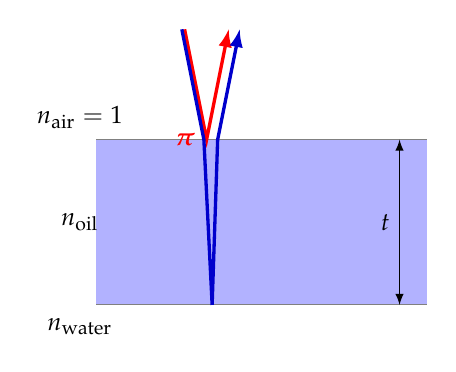
\begin{tikzpicture}[scale=.7]
      \fill[blue!30](0,0) rectangle(6,3);
      \draw[gray](0,0)--(6,0);
      \draw[gray](0,3)--(6,3);
      \draw[<->](5.5,0)--(5.5,3) node[midway,left]{\small  $t$};
      \draw[very thick,red,->]
      (1.6,5)--(2,3) node[left]{\small $\bm{\pi}$}--(2.4,5);
      \draw[very thick,blue!80!black,->]
      (1.55,5)--(1.95,3)--(2.1,0)--(2.2,3)--(2.6,5);
      \node at (-.3,1.5 ){\small $n_\text{oil}$};
      \node at (-.3,3.4){\small $n_\text{air}=1$};
      \node at (-.3,-.4){\small $n_\text{water}$};
    \end{tikzpicture}
  \end{center}
  Light travels through air and strikes a oil film (with
  $n_\text{oil}$). Below the oil film is water, which has a lower refractive
  index than oil ($n_\text{oil}>n_\text{water}$)
  \begin{itemize}
  \item Upper interface: Reflected light has a phase shift of \ang{180} ($\pi$)
    because $n_\text{air}<n_\text{oil}$ (fast to slow medium)
  \item Lower interface: Reflected light has no phase shifts (slow to fast
    medium)
  \end{itemize}
\end{frame}



\begin{frame}{Oil Film on Water}
  Beause there is only one phase shift, so like the soap bubble,
  \emph{constructive maxima} occurs if path difference is a half-number
  multiple of wavelength:

  \eq{-.22in}{
    \boxed{
      \frac{2n_\text{oil}t}{\lambda}=m+\frac12
    }
  }

  while \emph{destructive minima} if $\Gamma$ is a whole-number multiple of
  wavelength:

  \eq{-.22in}{
    \boxed{
      \frac{2n_\text{oil}t}\lambda=m
    }
  }

  where $m=0,1,2\ldots$, and assuming that the refractive index of the oil
  film is \emph{higher} than water.
\end{frame}



\begin{frame}{Anti-Reflection Coating}
  \begin{center}
    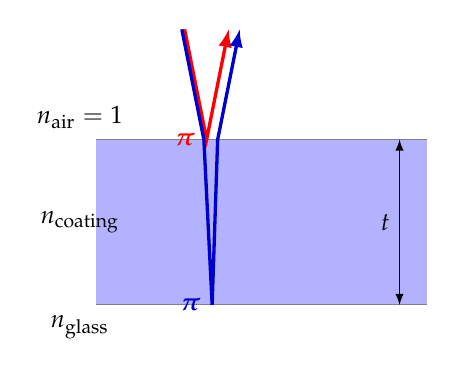
\begin{tikzpicture}[scale=.7]
      \fill[blue!30](0,0) rectangle(6,3);
      \draw[gray](0,0)--(6,0);
      \draw[gray](0,3)--(6,3);
      \draw[<->](5.5,0)--(5.5,3) node[midway,left]{\small$t$};
      \draw[very thick,red,->]
      (1.6,5)--(2,3) node[left]{\small $\bm{\pi}$}--(2.4,5);
      \draw[very thick,blue!80!black,->]
      (1.55,5)--(1.95,3)--(2.1,0) node[left]{\small $\bm{\pi}$}--
      (2.2,3)--(2.6,5);
      \node at (-.3,1.5 ){\small $n_\text{coating}$};
      \node at (-.3,3.4){\small $n_\text{air}=1$};
      \node at (-.3,-.4){\small $n_\text{glass}$};
    \end{tikzpicture}
  \end{center}
  
  \vspace{-.1in}Anti-reflective coating on eyeglasses and camera lenses
  has a refractive index lower than glass (but higher than air), i.e.:

  \eq{-.33in}{
    n_\text{air}<n_\text{coating}<n_\text{glass}
  }

  \vspace{-.13in}Light reflects with a phase shift of $\pi$ on both the upper
  and lower interfaces, because in both cases, the light is from fast to
  slow medium
\end{frame}




\begin{frame}{Anti-Reflection Coating}
  The interference conditions for anti-reflection coating is \emph{oppposite}
  to the soap bubble and oil film, because the phase shifts occur on both
  boundaries. \emph{Constructive maxima} occurs if path difference is a
  whole-number multiple of wavelength:

  \eq{-.22in}{
    \boxed{
      \frac{2n_\text{film}t}\lambda=m
    }
  }

  while \emph{destructive minima} occurs if path difference is a half-number
  multiple of wavelength:

  \eq{-.22in}{
    \boxed{
      \frac{2n_\text{film}t}\lambda=m+\frac12
    }
  }

  where $m=0,1,2\ldots$
\end{frame}
\end{document}
